\section{Trazado de rayos}

Si resolvemos las ecuaciones de Hamilton, podemos trazar la
trayectoria del rayo. Este procedimiento se llama trazado de rayos.
Demos algunos ejemplos.

\textbf{Ejemplo 1.} En un medio de velocidad constante, tenemos
\begin{equation}
    \omega(\mathbf{k}, \mathbf{r}) = v k = v \sqrt{k_x^2 + k_z^2}.
\end{equation}

La forma componente de las ecuaciones de Hamilton da:

\begin{equation}
    \frac{dx}{dt}
    = \frac{\partial \omega}{\partial k_x}
    = \frac{k_x v}{k}
    \quad \text{y} \quad \frac{dz}{dt}
    = -\frac{\partial \omega}{\partial k_z}
    = \frac{k_z v}{k},
\end{equation}

\begin{equation}
    \frac{d k_x}{dt} =-\frac{\partial \omega}{\partial x}
    = 0
    \quad \text{y} \quad \frac{dk_z}{dt}
    = -\frac{\partial \omega}{\partial z} = 0.
\end{equation}

Las ecuaciones 24 dicen que \( k_x \) y \( k_z \) son constantes.
Así,

\[ k = \sqrt{k_x^2 + k_z^2} = \text{constante}. \]

Integrando las ecuaciones 23, obtenemos las ecuaciones del rayo:

\begin{equation}
    x = \frac{k_x}{k} vt + x_0 \quad \text{y} \quad z
    = \frac{k_z}{k} vt + z_0,
\end{equation}

donde \( x_0 \) y \( z_0 \) son los valores de \( x \) y \( z \),
respectivamente, en \( t = 0 \). Así, el rayo está en la dirección
del vector de propagación constante \( (k_x, k_z) \).
Dado que \( k \) es la magnitud del vector de propagación,
vemos que tenemos una onda plana moviéndose con velocidad \( v \).

\textbf{Ejemplo 2. } Ahora consideremos un medio estratificado con
la relación de dispersión

\begin{equation}
    v(\mathbf{k}, \mathbf{r})
    = kv(z) = \sqrt{k_x^2 + k_z^2} \, v(z).
\end{equation}

En este caso, las ecuaciones de Hamilton son las cuatro ecuaciones:

\begin{equation}
    \frac{dx}{dt} = \frac{\partial v}{\partial k_x}
    = \frac{k_x v(z)}{k}, \quad \text{y} \quad \frac{dz}{dt}
    = \frac{\partial v}{\partial k_z} = \frac{k_x v(z)}{k},
\end{equation}

y

\begin{equation}
    \frac{dk_x}{dt} = -\frac{\partial \omega}{\partial x}
    = 0 \quad \text{y} \quad \frac{dk_z}{dt}
    = -\frac{\partial \omega}{\partial z}
    = k \frac{dv}{dz}.
\end{equation}

Dividiendo \( \frac{dx}{dt} \) por \( \frac{dz}{dt} \) en la ecuación
27, obtenemos

\begin{equation}
    \frac{dx}{dz} = \frac{\frac{dx}{dt}}{\frac{dz}{dt}}
    = \frac{\frac{\partial \omega}{\partial k_x}}
    {\frac{\partial \omega}{\partial k_z}} = \frac{k_x}{k_z}.
\end{equation}


Por lo tanto, los rayos están en la dirección del vector número de
onda \( \mathbf{k} \). La primera ecuación en 28 nos da
\( k_x = \text{constante} \). Ahora usamos nuestro resultado general
anterior de que la frecuencia es constante a lo largo de un rayo.
Por lo tanto, vemos que \( \frac{k_x}{v} = \text{constante} \)
a lo largo de un rayo en un medio estratificado. Si llamamos a
esta constante \( p_x \), entonces usamos la ecuación 26 y tenemos

\begin{equation}
    p_x = \frac{k_x}{\omega} = \frac{k_x}{kv(z)} = \text{constante}.
\end{equation}

Refiriéndonos a la Figura 3, definimos \( u(z) \) como el ángulo
entre el rayo y la vertical. Es decir, \( \sin \theta = k_x/k \) y
\( \cos \theta = k_z/k \).

\begin{figure}[h]
    \centering
    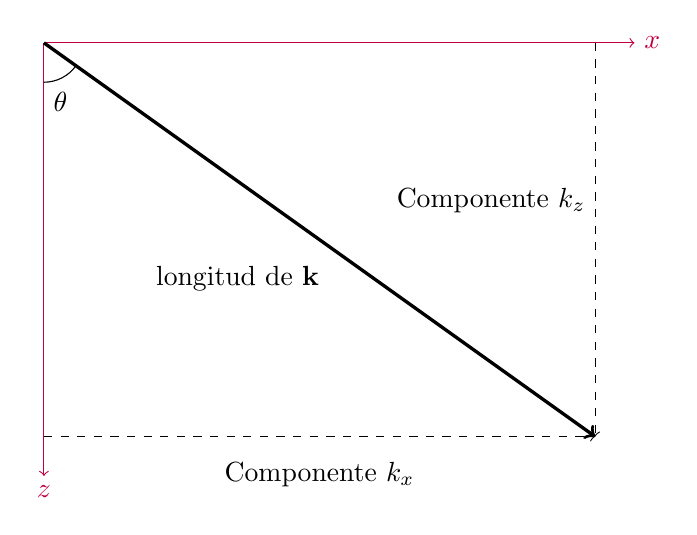
\begin{tikzpicture}
       % \draw[help lines] (0, 0) grid (7, -5);
       \draw [->, color=purple] (0, 0) -- (7.5, 0) node[right] {$x$};
       \draw [->, color=purple] (0, 0) -- (0, -5.5) node[below] {$z$};
       \draw [->, line width=1.2pt] (0, 0) -- (7, -5);
       \draw [->, dashed] (0, -5) -- (7, -5);
       \draw [->, dashed] (7, 0) -- (7, -5);
       \draw (0, -0.5) arc (-90:-35:0.5);
       \node [right] at (0, -0.75) {$\theta$};
       \node [below] at (3.5, -5.2) {Componente $k_x$};
       \node [left] at (7, -2) {Componente $k_z$};
       \node [right] at (1.3, -3) {longitud de $\mathbf{k}$};
   \end{tikzpicture}
   \caption{Definición del ángulo $\theta$.}
\end{figure}

Por lo tanto, la ecuación 30 se ve como la ley de Snell

\begin{gather}
    p_x = \frac{\sin \theta}{v(z)} = \text{constante}.
\end{gather}

Usando la ley de Snell, como se muestra en la ecuación 31, tenemos

\begin{gather}
    \frac{k_x}{k} = \sin \theta(z) = p_x v(z) \quad \text{y} \quad
    \frac{k_z}{k} = \cos \theta(z) = \sqrt{1 - p_x^2 v^2(z)}.
\end{gather}

Ahora integraremos la ecuación

\begin{equation}
    \frac{dx}{dz} = \frac{k_x}{k_z} =
    \frac{p_x v(z)}{\sqrt{1 - p_x^2 v^2(z)}}.
\end{equation}

Haciéndolo, obtenemos la llamada ecuación de distancia horizontal

\begin{equation}
    x = \int_0^z \frac{p_x v(z) \, dz}{\sqrt{1 - p_x^2 v^2(z)}}.
\end{equation}

También podemos integrar la segunda ecuación de Hamilton mostrada en la
ecuación 27,
\begin{equation}
    \frac{dz}{dt} = \frac{k_z v(z)}{k} = \sqrt{1 - p_x^2 v^2(z)} \, v(z),
\end{equation}

para obtener la llamada ecuación de tiempo

\begin{equation}
    t = \int_0^z \frac{dz}{v(z) \sqrt{1 - p_x^2 v^2(z)}}.
\end{equation}

La ecuación de tiempo (ecuación 36) junto con la ecuación de distancia
horizontal (ecuación 34) componen la llamada relación tiempo-distancia
para el rayo. Es decir, las ecuaciones 36 y 34 dan la llamada curva
tiempo-distancia como función del parámetro \( p_x \) de las ondas que
se originan en \( z = 0 \) y viajan a una profundidad
\( z = \text{constante} \).

Como se muestra en la Figura 4, cada punto en la curva tiempo-distancia
está determinado por un valor particular de \( p_x \). Dado que cada
valor de \( p_x \) designa un rayo, la curva tiempo-distancia resume la
información de todos los rayos que alcanzan la profundidad \( z \).

Podemos escribir la ecuación de distancia horizontal en otra forma.
La primera de las ecuaciones de Hamilton (ecuaciones 27) es

\begin{equation}
    \frac{dx}{dt} = \frac{k_x v(z)}{k} = v(z) \sin \theta(z) \quad
    \text{(a lo largo de un rayo)}.
\end{equation}

Sin embargo, la ecuación de Snell es \(\sin \theta(z) = p_x v(z)\).
Así, la ecuación 37 es

\begin{equation}
    \frac{dx}{dt} = p_x v^2(z) \quad \text{(a lo largo de un rayo)},
\end{equation}


por lo que la forma \textit{alternativa requerida de la ecuación de
distancia horizontal es}

\begin{equation}
    x = \int_0^t p_x v^2(z) \, dt = p_x \int_0^t v^2(z) \, dt.
\end{equation}

Recuerde que las ecuaciones de Hamilton (ecuaciones 27 y 28) se aplican
para trayectorias a lo largo de un rayo. Un ejemplo perfecto es la
ecuación 38 anterior.

Por otro lado, la curva tiempo-distancia se aplica a todos los rayos
(cada uno caracterizado por un valor de \( p_x \)) que se extienden hasta
una profundidad dada \( z = \text{constante} \). Ahora, queremos mostrar
que

\begin{equation}
    \frac{dx}{dt} = \frac{1}{p_x}
    \quad \text{(a lo largo de la curva tiempo-distancia)}.
\end{equation}

% TODO: Insert figure 4 here

El argumento geométrico, como se muestra en la Figura 5, puede ser
utilizado. Del diagrama, vemos que

\begin{equation}
    \frac{dx}{v \, dt} = \frac{1}{\sin \theta}.
\end{equation}

Usando la ley de Snell \( p_x = \frac{\sin \theta}{v} \), obtenemos
el resultado requerido, la ecuación 40. Así, la pendiente de la curva
tiempo-distancia es igual al parámetro de Snell \( p_x \); es decir,

\begin{equation}
    \frac{dt}{dx} = p_x
    \quad \text{(a lo largo de la curva tiempo-distancia)}.
\end{equation}

La importancia del parámetro \( p_x \) se realiza tomando \( z = 0 \)
en la ecuación de Snell,

\begin{equation}
    p_x = \frac{\sin \theta(0)}{v(0)}.
\end{equation}

La ecuación 43 muestra que \( p_x \) es proporcional al seno del ángulo
de incidencia \(\theta(0)\) del rayo en la superficie \( z = 0 \).

En el caso de velocidad constante, es decir,
\( v(z) = V = \text{constante} \), la curva tiempo-distancia es la
hipérbola

\begin{equation}
    V^2 t^2 - x^2 = z^2 = \text{constante}.
\end{equation}

En el caso de un medio estratificado con la función de velocidad
\( v(z) \), generalmente la forma de la curva tiempo-distancia se
asemejará a una hipérbola (ver Figura 6). Supongamos que un pulso en
el tiempo \( t = 0 \) se propaga hacia afuera desde una fuente puntual
en \( z = 0 \). A alguna profundidad (o, alternativamente, altura)
\( z = \text{constante} \), medimos el tiempo de llegada \( t \)
del pulso como una función de la coordenada horizontal \( x \).
El resultado es la curva tiempo-distancia, como la mostrada en la
Figura 5. Supongamos que ahora ajustamos la curva tiempo-distancia a
la hipérbola

% TODO: Insert figure 5 here
% TODO: Insert figure 6 here

La velocidad constante \(V\) se determina de manera que proporcione el
mejor ajuste. La pregunta es: ¿cómo se relaciona la velocidad constante
ajustada \(V\) con la función de velocidad variable \(v(z)\)?
Si diferenciamos la ecuación 44 para la hipérbola, obtenemos

\begin{equation}
    2V^2 t \, dt - 2x \, dx = 0 ,
\end{equation}
así que

\begin{equation}
    \frac{dt}{dx} = \frac{x}{t V^2} \text{ (en la hipérbola)} .
\end{equation}

Sin embargo, en la curva tiempo-distancia, tenemos
\( \frac{dt}{dx} = p_x \). Así que igualamos las dos derivadas
para obtener

\begin{equation}
    p_x = \frac{x}{t V^2} .
\end{equation}

Así, el valor requerido de \( V^2 \) es igual a \( \frac{x}{p_x t} \).
Si resolvemos la ecuación 47 para \( V \) y hacemos uso de la ecuación
39, obtenemos

\begin{equation}
    V^2 = \frac{x}{p_x t} = \frac{1}{t} \int_0^t v^2(z) \, dt .
\end{equation}

La ecuación 48 dice que \( V^2 \) es el valor cuadrático medio de
\( v(z) \) a lo largo de la trayectoria del rayo. Así, si ajustamos
la curva tiempo-distancia mediante una hipérbola, la velocidad \(V\)
que obtenemos es la velocidad cuadrática media (RMS) dada por

\begin{equation}
    V = V_{\text{RMS}} = \sqrt{\frac{1}{t} \int_0^t v^2(z) \, dt} .
\end{equation}
En otras palabras, podemos decir que, si necesitamos una velocidad
promedio para caracterizar el medio estratificado hasta una profundidad
\(z\), una excelente elección es la velocidad cuadrática media.